\chapter{SP2-CU4 Desasignar unidades de aprendizaje a un analista }

\begin{UseCase}{SP2-CU4}{Desasignar unidades de apendizaje a un analista}{El usuario jefe de desarrollo e innovación curricular podrá modificar a los analistas encargados de una unidad de aprendizaje.}
		\UCitem{Versión}{\color{Gray}1.0}
		\UCitem{Autor}{\color{Gray}Parra Garcilazo Cinthya Dolores}
		\UCitem{Supervisa}{\color{Gray}}
		\UCitem{Actor}{\hyperlink{Usuario}{Jefe de Desarrollo e Innovación Curricular}}
		\UCitem{Propósito}{Asignar el acceso a una unidad de aprendizaje a otro analista.}
		\UCitem{Entradas}{Las entradas para modificar una unidad de aprendizaje a otro analista son:
          \begin{itemize}
          	\item Analista
          \end{itemize}
        }
		\UCitem{Origen}{Teclado, mouse.}
		\UCitem{Salidas}{
        	\begin{itemize}
        	   \item Mensaje Operación realizada
        	\end{itemize}
        }
		\UCitem{Destino}{Pantalla.}
		\UCitem{Precondiciones}{ Debe haber una analista ya asignado a esa revisión.}
		\UCitem{Postcondiciones}{El nuevo analista asignado puede acceder a la propuesta de unidad de aprendizaje y realizar los comentarios pertinenetes. El analista previo no puede acceder a la información.}
		\UCitem{Errores}{}
		\UCitem{Estado}{Revisión.}
		\UCitem{Observaciones}{}
\end{UseCase}

%--------------------------- CU TRAYECTORIA PRINCIPAL -------------------------
\begin{UCtrayectoria}{Principal}


    \UCpaso Muestra la interfaz de usuario \IUref{GestionEncargado}
    \UCpaso [\UCactor] Presiona el botón \IUbutton {Editar}
    \UCpaso Activa los campos de fecha y analista.
    \UCpaso [\UCactor] Selecciona el campo de analista.
    \UCpaso Despliega la lista de analistas registrados en la base de datos.
    \UCpaso[\UCactor] Selecciona una opcion.
    \UCpaso [\UCactor] Presiona el botón \IUbutton {Confirmar}
    \UCpaso Modifica en la base de datos al analista asignado para la revisión de la unidad de aprendizaje
    \UCpaso Muestra el mensaje \MSGref {MSG1}
    \UCpaso[\UCactor] Presiona el botón \IUbutton {Aceptar}

\end{UCtrayectoria}



%------------------------ Pantallas de este caso de uso -------------------------
\chapter{Pantallas}
 \begin{figure}
  \centering
    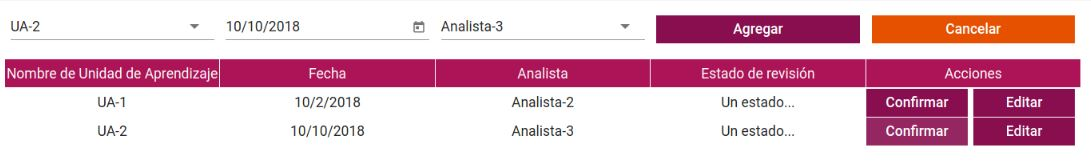
\includegraphics[width=0.7\textwidth]{DCU/SP2/Pantallas/GestionEncargado}
  \caption{SP2-IU-GestionEncargado}
  \label{SP2-IU-GestionEncargado}
\end{figure}

%------------------------ Mensajes de este caso de uso -------------------------
\chapter{Mensajes}
 \begin{figure}
  \centering
    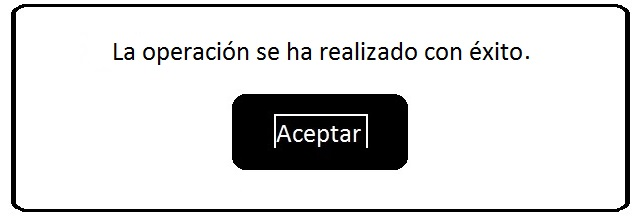
\includegraphics[width=0.7\textwidth]{DCU/SP2/mensajes/MSG1}
   \caption{SP2-MSG1}
  \label{SP2-MSG1}
\end{figure}


